\documentclass{beamer}
\usefonttheme[onlymath]{serif}
\usepackage[T1]{fontenc}
\usepackage[utf8]{inputenc}
\usepackage[english]{babel}
\usepackage{amsmath}
\usepackage{amssymb}
\usepackage{amsthm}
\usepackage{gensymb}
\usepackage{parskip}
\usepackage{mathtools}
\usepackage{listings}
\usepackage{hyperref}
\usepackage{graphicx}
\usepackage{color}
\usepackage{enumerate}
\usepackage{tikz}
\usetikzlibrary{calc}
\usetikzlibrary{positioning}
\usetikzlibrary{angles}
\usetikzlibrary{shapes}
\usetikzlibrary{arrows}
\usepackage{verbatim}
\usepackage{multicol}
\usepackage{array}
\usepackage{minted}
\parskip 0pt


\DeclareMathOperator{\lcm}{lcm}
\newcommand\floor[1]{\left\lfloor#1\right\rfloor}
\newcommand\ceil[1]{\left\lceil#1\right\rceil}
\newcommand\abs[1]{\left|#1\right|}
\newcommand\p[1]{\left(#1\right)}
\newcommand\sqp[1]{\left[#1\right]}
\newcommand\cp[1]{\left\{#1\right\}}
\newcommand\norm[1]{\left\lVert#1\right\rVert}
\renewcommand\Im{\operatorname{Im}}
\renewcommand\Re{\operatorname{Re}}

\usetheme{metropolis}
\definecolor{dark yellow}{rgb} {0.6,0.6,0.0}
\definecolor{dark green}{rgb} {0.0,0.6,0.0}

\graphicspath{{myndir/}}

\title{Segment Tree}
\author{Arnar Bjarni Arnarson}
\institute{\href{http://ru.is/td}{School of Computer Science} \\[2pt] \href{http://ru.is}{Reykjavík University}}
\titlegraphic{\hfill\includegraphics[height=0.6cm]{kattis}}

\begin{document}
\maketitle

\begin{frame}[plain]{Range queries}
    \vspace{30pt}
    \begin{itemize}
        \item<1-> We have an array $A$ of size $n$.
        \item<2-> Given $i,j$, we want to answer:
            \begin{itemize}
                \item<3-> $\mathrm{max}(A[i],A[i+1],\ldots,A[j-1],A[j])$
                \item<4-> $\mathrm{min}(A[i],A[i+1],\ldots,A[j-1],A[j])$
                \item<5-> $\mathrm{sum}(A[i],A[i+1],\ldots,A[j-1],A[j])$
            \end{itemize}
        \item<6-> We want to answer these queries efficiently, or in other words, without looking through all elements.
        \item<7-> Sometimes we also want to update elements.
    \end{itemize}
\end{frame}

\begin{frame}[plain,fragile]{Segment Tree}
    \begin{itemize}
        \item<1-> We create a perfect binary tree where the leaves are the elements of the array.
        \item<2-> Then each internal vertex is the sum of the values below it.
        \item<3-> Then we have $\mathcal{O}(n)$ nodes and each query can be pieced together from $\mathcal{O}(\log(n))$ node values.
        \item<4-> We travel down the tree looking for the left and right end points, adding intervals that are completely inside our query range.
        \item<5-> When we update a value we only need to update the parents of that node up to the root, at most $\mathcal{O}(\log(n))$ nodes.
    \end{itemize}
\end{frame}

\begin{frame}[plain]{Drawn Segment Tree, $n = 4$}
	\begin{center}
		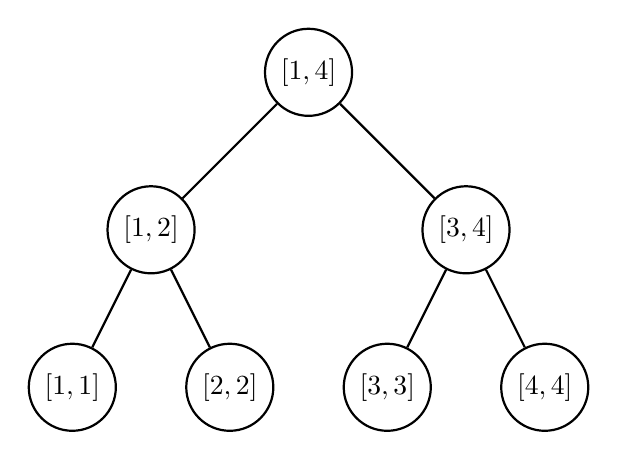
\begin{tikzpicture}
			\node[draw, circle, thick] (1) at (0,4) {$[1, 4]$};

			\node[draw, circle, thick] (2) at (-2,2) {$[1, 2]$};
			\node[draw, circle, thick] (3) at (2,2) {$[3, 4]$};

			\node[draw, circle, thick] (4) at (-3,0) {$[1, 1]$};
			\node[draw, circle, thick] (5) at (-1,0) {$[2, 2]$};
			\node[draw, circle, thick] (6) at (1,0) {$[3, 3]$};
			\node[draw, circle, thick] (7) at (3,0) {$[4, 4]$};

			\path[draw, thick] (1) -- (2);
			\path[draw, thick] (1) -- (3);
			\path[draw, thick] (2) -- (4);
			\path[draw, thick] (2) -- (5);
			\path[draw, thick] (3) -- (6);
			\path[draw, thick] (3) -- (7);
        \end{tikzpicture}
    \end{center}
\end{frame}

\begin{frame}[plain]{Drawn Segment Tree, $n = 7$}
	\begin{center}
		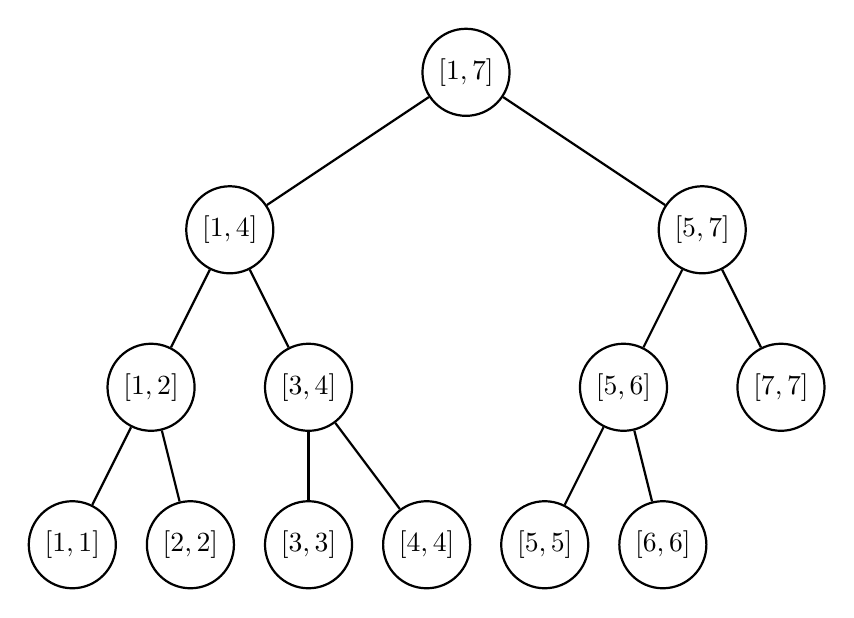
\begin{tikzpicture}
			\node[draw, circle, thick] (1) at (0,6) {$[1, 7]$};

			\node[draw, circle, thick] (2) at (-3,4) {$[1, 4]$};
			\node[draw, circle, thick] (3) at (3,4) {$[5, 7]$};

			\node[draw, circle, thick] (4) at (-4,2) {$[1, 2]$};
			\node[draw, circle, thick] (5) at (-2,2) {$[3, 4]$};
			\node[draw, circle, thick] (6) at (2,2) {$[5, 6]$};
			\node[draw, circle, thick] (7) at (4,2) {$[7, 7]$};

			\node[draw, circle, thick] (8) at (-5,0) {$[1, 1]$};
			\node[draw, circle, thick] (9) at (-3.5,0) {$[2, 2]$};
			\node[draw, circle, thick] (10) at (-2,0) {$[3, 3]$};
			\node[draw, circle, thick] (11) at (-0.5,0) {$[4, 4]$};
			\node[draw, circle, thick] (12) at (1,0) {$[5, 5]$};
			\node[draw, circle, thick] (13) at (2.5,0) {$[6, 6]$};

			\path[draw, thick] (1) -- (2);
			\path[draw, thick] (1) -- (3);
			\path[draw, thick] (2) -- (4);
			\path[draw, thick] (2) -- (5);
			\path[draw, thick] (3) -- (6);
			\path[draw, thick] (3) -- (7);
			\path[draw, thick] (4) -- (8);
			\path[draw, thick] (4) -- (9);
			\path[draw, thick] (5) -- (10);
			\path[draw, thick] (5) -- (11);
			\path[draw, thick] (6) -- (12);
			\path[draw, thick] (6) -- (13);
        \end{tikzpicture}
    \end{center}
\end{frame}

\begin{frame}[plain,fragile]{Segment Tree - Code}
    \begin{minted}[fontsize=\scriptsize]{cpp}
struct segment_tree {
    segment_tree *left, *right;
    int from, to, value;
    segment_tree(int from, int to)
        : from(from), to(to), left(NULL), right(NULL), value(0) { }
};

segment_tree* build(const vector<int> &arr, int l, int r) {
    if (l > r) return NULL;
    segment_tree *res = new segment_tree(l, r);
    if (l == r) {
        res->value = arr[l];
    } else {
        int m = (l + r) / 2;
        res->left = build(arr, l, m);
        res->right = build(arr, m + 1, r);
        if (res->left != NULL) res->value += res->left->value;
        if (res->right != NULL) res->value += res->right->value;
    }
    return res;
}
    \end{minted}
\end{frame}

\begin{frame}[plain]{Updates}
	\begin{center}
		\begin{tikzpicture}
			\only<all:1-2, 14-15, 24-> { \node[draw, circle, thick] (1) at (0,6) {\phantom{xxx}}; }
			\only<all:3-13, 16-23> { \node[draw, circle, thick, red] (1) at (0,6) {\phantom{xxx}}; }


			\only<all:1-3, 12-> { \node[draw, circle, thick] (2) at (-3,4) {\phantom{xxx}}; }
			\only<all:4-11> { \node[draw, circle, thick, red] (2) at (-3,4) {\phantom{xxx}}; }

			\only<all:1-16, 22-> { \node[draw, circle, thick] (3) at (3,4) {\phantom{xxx}}; }
			\only<all:17-21> { \node[draw, circle, thick, red] (3) at (3,4) {\phantom{xxx}}; }


			\only<all:1-> { \node[draw, circle, thick] (4) at (-4,2) {\phantom{xxx}}; }

			\only<all:1-4, 10-> { \node[draw, circle, thick] (5) at (-2,2) {\phantom{xxx}}; }
			\only<all:5-9> { \node[draw, circle, thick, red] (5) at (-2,2) {\phantom{xxx}}; }

			\only<all:1-> { \node[draw, circle, thick] (6) at (2,2) {\phantom{xxx}}; }

			\only<all:1-17, 20-> { \node[draw, circle, thick] (7) at (4,2) {\phantom{xxx}}; }
			\only<all:18-19> { \node[draw, circle, thick, red] (7) at (4,2) {\phantom{xxx}}; }


			\only<all:1-> { \node[draw, circle, thick] (8) at (-5,0) {\phantom{xxx}}; }

			\only<all:1-> { \node[draw, circle, thick] (9) at (-3.5,0) {\phantom{xxx}}; }

			\only<all:1-> { \node[draw, circle, thick] (10) at (-2,0) {\phantom{xxx}}; }

			\only<all:1-5, 8-> { \node[draw, circle, thick] (11) at (-0.5,0) {\phantom{xxx}}; }
			\only<all:6-7> { \node[draw, circle, thick, red] (11) at (-0.5,0) {\phantom{xxx}}; }

			\only<all:1-> { \node[draw, circle, thick] (12) at (1,0) {\phantom{xxx}}; }

			\only<all:1-> { \node[draw, circle, thick] (13) at (2.5,0) {\phantom{xxx}}; }

			\path[draw, thick] (1) -- (2);
			\path[draw, thick] (1) -- (3);
			\path[draw, thick] (2) -- (4);
			\path[draw, thick] (2) -- (5);
			\path[draw, thick] (3) -- (6);
			\path[draw, thick] (3) -- (7);
			\path[draw, thick] (4) -- (8);
			\path[draw, thick] (4) -- (9);
			\path[draw, thick] (5) -- (10);
			\path[draw, thick] (5) -- (11);
			\path[draw, thick] (6) -- (12);
			\path[draw, thick] (6) -- (13);


			\only<all:2-14> { \node at (-3,6) {\texttt{update(3, 7)}}; }
			\only<all:15-24> { \node at (-3,6) {\texttt{update(6, -12)}}; }
			\only<all:25-> { \node at (-3,6) {}; }

			\only<all:1-12> { \node at (0,6) {$40$}; }
			\only<all:13-22> { \node at (0,6) {$47$}; }
			\only<all:23-> { \node at (0,6) {$35$}; }

			\only<all:1-10> { \node at (-3,4) {$16$}; }
			\only<all:11-> { \node at (-3,4) {$23$}; }

			\only<all:1-20> { \node at (3,4) {$24$}; }
			\only<all:21-> { \node at (3,4) {$12$}; }

			\only<all:1-> { \node at (-4,2) {$5$}; }

			\only<all:1-8> { \node at (-2,2) {$11$}; }
			\only<all:9-> { \node at (-2,2) {$18$}; }

			\only<all:1-> { \node at (2,2) {$17$}; }

			\only<all:1-18> { \node at (4,2) {$7$}; }
			\only<all:19-> { \node at (4,2) {$-5$}; }

			\only<all:1-> { \node at (-5,0) {$3$}; }

			\only<all:1-> { \node at (-3.5,0) {$2$}; }

			\only<all:1-> { \node at (-2,0) {$9$}; }

			\only<all:1-6> { \node at (-0.5,0) {$2$}; }
			\only<all:7-> { \node at (-0.5,0) {$9$}; }

			\only<all:1-> { \node at (1,0) {$9$}; }

			\only<all:1-> { \node at (2.5,0) {$8$}; }
        \end{tikzpicture}
    \end{center}
\end{frame}

\begin{frame}[plain,fragile]{Updating a Segment Tree - Code}
    \vspace{40pt}
    \begin{minted}[fontsize=\scriptsize]{cpp}
int update(segment_tree *tree, int i, int val) {
    if (tree == NULL) return 0;
    if (tree->to < i) return tree->value;
    if (i < tree->from) return tree->value;
    if (tree->from == tree->to && tree->from == i) {
        tree->value = val;
    } else {
        tree->value = update(tree->left, i, val) + update(tree->right, i, val);
    }
    return tree->value;
}
    \end{minted}
\end{frame}

\begin{frame}[plain]{Querying}
	\begin{center}
		\begin{tikzpicture}
			\only<all:2-9> { \node at (-3,6) {\texttt{query(1, 7)}}; }
			\only<all:10-17> { \node at (-3,6) {\texttt{query(1, 2)}}; }

			\only<all:8> { \node at (-3,5.5) {\texttt{= 2 + 18 + 12}}; }
			\only<all:9> { \node at (-3,5.5) {\texttt{= 32}}; }
			\only<all:16> { \node at (-3,5.5) {\texttt{= 2 + 9}}; }
			\only<all:17> { \node at (-3,5.5) {\texttt{= 11}}; }



			\only<all:1-2, 4-10, 12-> { \node[draw, circle, thick] (1) at (0,6) {\phantom{xxx}}; }
			\only<all:3, 11> { \node[draw, circle, thick, red] (1) at (0,6) {\phantom{xxx}}; }


			\only<all:1-3, 5-11, 13-> { \node[draw, circle, thick] (2) at (-3,4) {\phantom{xxx}}; }
			\only<all:4, 12> { \node[draw, circle, thick, red] (2) at (-3,4) {\phantom{xxx}}; }

			\only<all:1-3, 10-> { \node[draw, circle, thick] (3) at (3,4) {\phantom{xxx}}; }
			\only<all:4> { \node[draw, circle, thick, red] (3) at (3,4) {\phantom{xxx}}; }
			\only<all:5-9> { \node[draw, circle, thick, blue] (3) at (3,4) {\phantom{xxx}}; }


			\only<all:1-4, 6-12, 14-> { \node[draw, circle, thick] (4) at (-4,2) {\phantom{xxx}}; }
			\only<all:5, 13> { \node[draw, circle, thick, red] (4) at (-4,2) {\phantom{xxx}}; }

			\only<all:1-4, 10-12, 14-> { \node[draw, circle, thick] (5) at (-2,2) {\phantom{xxx}}; }
			\only<all:5, 13> { \node[draw, circle, thick, red] (5) at (-2,2) {\phantom{xxx}}; }
			\only<all:6-9> { \node[draw, circle, thick, blue] (5) at (-2,2) {\phantom{xxx}}; }

			\only<all:1-> { \node[draw, circle, thick] (6) at (2,2) {\phantom{xxx}}; }

			\only<all:1-> { \node[draw, circle, thick] (7) at (4,2) {\phantom{xxx}}; }


			\only<all:1-> { \node[draw, circle, thick] (8) at (-5,0) {\phantom{xxx}}; }

			\only<all:1-5, 10-13, 18-> { \node[draw, circle, thick] (9) at (-3.5,0) {\phantom{xxx}}; }
			\only<all:6, 14> { \node[draw, circle, thick, red] (9) at (-3.5,0) {\phantom{xxx}}; }
			\only<all:7-9, 15-17> { \node[draw, circle, thick, blue] (9) at (-3.5,0) {\phantom{xxx}}; }

			\only<all:1-13, 18-> { \node[draw, circle, thick] (10) at (-2,0) {\phantom{xxx}}; }
			\only<all:14> { \node[draw, circle, thick, red] (10) at (-2,0) {\phantom{xxx}}; }
			\only<all:15-17> { \node[draw, circle, thick, blue] (10) at (-2,0) {\phantom{xxx}}; }

			\only<all:1-> { \node[draw, circle, thick] (11) at (-0.5,0) {\phantom{xxx}}; }

			\only<all:1-> { \node[draw, circle, thick] (12) at (1,0) {\phantom{xxx}}; }

			\only<all:1-> { \node[draw, circle, thick] (13) at (2.5,0) {\phantom{xxx}}; }

			\path[draw, thick] (1) -- (2);
			\path[draw, thick] (1) -- (3);
			\path[draw, thick] (2) -- (4);
			\path[draw, thick] (2) -- (5);
			\path[draw, thick] (3) -- (6);
			\path[draw, thick] (3) -- (7);
			\path[draw, thick] (4) -- (8);
			\path[draw, thick] (4) -- (9);
			\path[draw, thick] (5) -- (10);
			\path[draw, thick] (5) -- (11);
			\path[draw, thick] (6) -- (12);
			\path[draw, thick] (6) -- (13);

			\node at (0,6) {$35$};
			\node at (-3,4) {$23$};
			\node at (3,4) {$12$};
			\node at (-4,2) {$5$};
			\node at (-2,2) {$18$};
			\node at (2,2) {$17$};
			\node at (4,2) {$-5$};
			\node at (-5,0) {$3$};
			\node at (-3.5,0) {$2$};
			\node at (-2,0) {$9$};
			\node at (-0.5,0) {$9$};
			\node at (1,0) {$9$};
			\node at (2.5,0) {$8$};
        \end{tikzpicture}
    \end{center}
\end{frame}


\begin{frame}[plain,fragile]{Querying a Segment Tree - Code}
    \vspace{50pt}
    \begin{minted}[fontsize=\scriptsize]{cpp}
int query(segment_tree *tree, int l, int r) {
    if (tree == NULL) return 0;
    if (l <= tree->from && tree->to <= r) return tree->value;
    if (tree->to < l) return 0;
    if (r < tree->from) return 0;
    return query(tree->left, l, r) + query(tree->right, l, r);
}
    \end{minted}
\end{frame}

\begin{frame}[plain]{Segment Tree}
    \begin{itemize}
        \item<1-> Simple to use Segment Trees for $\min$, $\max$, $\gcd$, and other similar operators, basically the same code.
        \item<2-> Any associative operator will work.
        \item<3-> So any operator $f$ such that $f(a, f(b, c)) = f(f(a, b), c)$ for all $a, b, c$.
    \end{itemize}
\end{frame}

\begin{frame}[plain]{Example problem: Movie Collection}
    \begin{itemize}
        \item https://open.kattis.com/problems/moviecollection
    \end{itemize}
\end{frame}

\subsection*{Range updates and queries}

\begin{frame}[plain]{Range updates}
    \begin{itemize}
        \item<1-> So far, we have only allowed updates to affect a single element.
        \item<2-> Might want to update multiple elements simultaneously, iterating for each is expensive.
        \item<3-> Example: For all indices from $4$ to $7$ add $13$.
        \item<4-> Can we make use of our segmented structure to update all indices in range $[l, r]$?
        \item<5-> Lazy people tend to find efficient ways of doing all that \textbf{needs} to be done, but no more.
        \item<6-> After updating a value, there is no guarantee you will use the updated value afterwards.
        \item<7-> Idea: Be lazy and procrastinate changes until they are needed!
    \end{itemize}
\end{frame}

\begin{frame}[plain]{Lazy propagation}
    \begin{itemize}
        \item<1-> Add another variable for each node, storing the lazy value
        \item<2-> Follow same steps as querying in order to update, applying the update if the node is completely within the range.
        \item<3-> When making updates, do not change the original data variable, but rather the lazy variable.
        \item<4-> When looking at a node, apply the lazy value to the node
        \item<5-> After applying, push the lazy value to the two child nodes
        \item<6-> Reset the lazy value.
        \item<7-> Traverse to child nodes if needed.
    \end{itemize}
\end{frame}

\begin{frame}[plain]{Code example}
    See implementation example, for example \href{https://github.com/keppnisforritun/aflv_slides/tree/main/datastructures/lazy_propagation_segment_tree.cpp}{here}.
\end{frame}

\end{document}
